\documentclass[11pt]{article} % use larger type; default would be 10pt

\usepackage[utf8]{inputenc} % set input encoding (not needed with XeLaTeX)
\usepackage{geometry} % to change the page dimensions
\geometry{a4paper} % or letterpaper (US) or a5paper or....
\usepackage{graphicx} % support the \includegraphics command and options
\usepackage{float}
% \usepackage[parfill]{parskip} % Activate to begin paragraphs with an empty line rather than an indent
\usepackage{booktabs} % for much better looking tables
\usepackage{array} % for better arrays (eg matrices) in maths
\usepackage{paralist} % very flexible & customisable lists (eg. enumerate/itemize, etc.)
\usepackage{verbatim} % adds environment for commenting out blocks of text & for better verbatim
\usepackage{subfig} % make it possible to include more than one captioned figure/table in a single float

\usepackage{fancyhdr} % This should be set AFTER setting up the page geometry
\pagestyle{fancy} % options: empty , plain , fancy
\renewcommand{\headrulewidth}{0pt} % customise the layout...
\lhead{}\chead{}\rhead{}
\lfoot{}\cfoot{\thepage}\rfoot{}

\usepackage{sectsty}
\allsectionsfont{\sffamily\mdseries\upshape} % (See the fntguide.pdf for font help)

\usepackage[nottoc,notlof,notlot]{tocbibind} % Put the bibliography in the ToC
\usepackage[titles,subfigure]{tocloft} % Alter the style of the Table of Contents
\renewcommand{\cftsecfont}{\rmfamily\mdseries\upshape}
\renewcommand{\cftsecpagefont}{\rmfamily\mdseries\upshape} % No bold!

%%%%%%%%%%%%%%%%%%%%%%%%%%%%%%%%%%%%%%%%%%%%%%%%%%

\title{UniVRPNity Documentation}
\author{Quentin Petit and Clément Grellier}
\date{}
\begin{document}
\maketitle

\section{Features}

\begin{itemize}
 \item Manage Analog, Button and Tracker remote.
 \item A syntax very close to C++ native client and VrpnNET client.
 \item Provide Unity MonoBehaviour scripts and editors for Analog, Button and Tracker remote.
 \item Provide concretes examples with these scripts (Translation, Rotation, Scale, Animation)
\end{itemize}


\begin{figure}[H]
	\begin{center}
	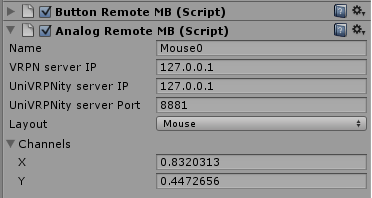
\includegraphics{UnityScript.png}
	\caption{MonoBehaviour remote of the mouse during execution.}
	\end{center}
\end{figure}

\section{Why using UniVRPNity?}

\subsection{VrpnNET}
VRPN is coding in C++ but free version of Unity only accept C\# ,  a modified JavaScript and Boo language.
After a few research we hopefully found VrpnNET a VRPN wrapper in C\#. 
But when we try to incorporate it in Unity it throw a native DLL error. 
Indeed! Free Unity version do not accept C++ wrapper.

\subsection{UIVA}
Then we found UIVA which create an intermediary between the VRPN wrapper and a full C\# client which is accepted by Unity.
However UIVA does not fit our needs because it is peripheral dependent. For instance to recover DTrack information, 
we had to modify the UIVA server and created a particular case for the DTrack data.

\subsection{VRPNWrapper}

\begin{figure}[H]
   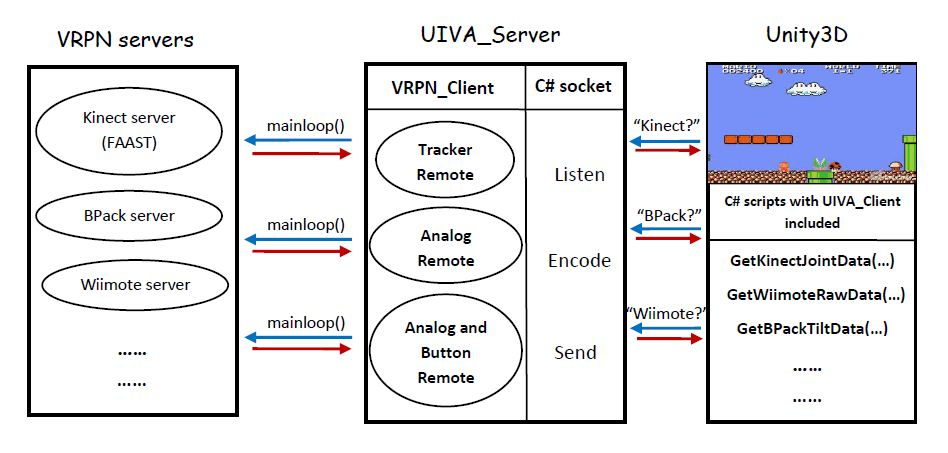
\includegraphics[scale=0.7]{UIVA_Framework.JPG}
   \caption{UIVA architecture.}
\end{figure}

\subsection{Full C\# client}

We also tried to write a full C\# from scratch but communication with a VRPN server is very hard :
\begin{itemize}
	\item There is no network specification of VRPN
	\item VRPN event are binary serialize with C++ type and depend of the VRPN event type (button, analog, tracker)
\end{itemize}
But we found a way and it worked for button (keyboard), analog (mouse) et tracker (DTrack) but this method wasn't safe and reliable. 
\begin{itemize}
	\item VRPN server send us all information from all peripheral with no easy way to distinguished them
	\item Parse an unknown frame except for it size is awkward
\end{itemize}

\subsection{UniVRPNity}
The only reliable solution was UIVA.
So we start from UIVA and rewrite a full middle server and a full C\# client.
It became a true intermediary, because VRPN event are sent directly to client (with a C\# conversion).

\section{UniVRPNity archictecture}

\begin{figure}[H]
	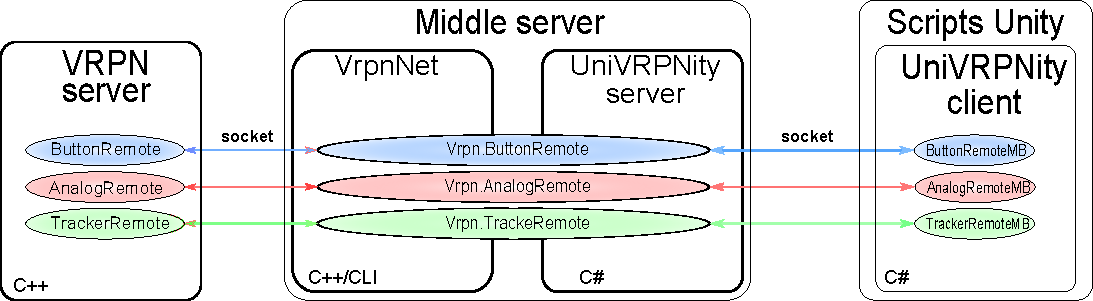
\includegraphics[scale=0.8]{UniVRPNity.pdf} 
	\caption{UniVRPNity architecture.}
\end{figure}


\section{How UniVRPNity work?}

\subsection{Requirement}
\begin{itemize}
	\item A running VRPN server which listening peripherals
      \item A running UniVRPNity server
\end{itemize}

\subsection{Initialization stage}
\begin{itemize}
	\item A remote client is created in a RemoteMB Start() method
	\item Client ask to the UniVRPNity server to pass through VRPN event of a named and typed device ("Mouse0@localhost\#Analog" are sent as handshake.)
      \item UniVRPNity server ask the same thing to the VRPN server
\end{itemize}

\subsection{Iterative stage : For each detected event}
\begin{itemize}
      \item VRPN server sent to UniVRPNity server all data of the event 
	\item UniVRPNity server convert these data in full C\# event and transfer them to the concerned client
	\item Client receive these data from socket and directly store it into a buffer (asynchronous)
	\item On next Update(), buffer are flushed into client callback (synchronous)
\end{itemize}



\begin{figure}[H]
	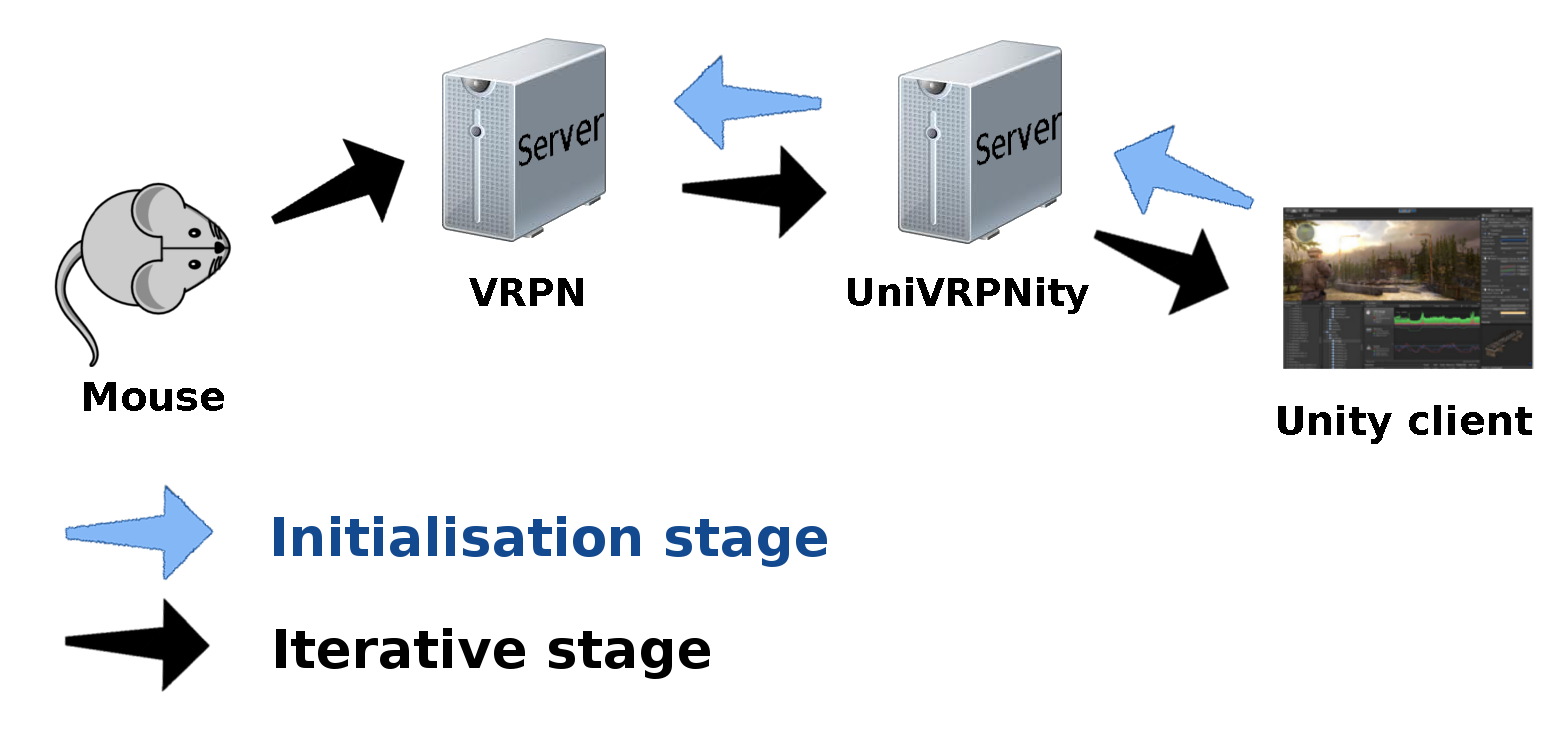
\includegraphics[scale=0.3]{UniVRPNityOrder.png} 
	\caption{UniVRPNity architecture.}
\end{figure}


\section{How to use UniVRPNity?}

\subsection{Compile projects}
	\begin{itemize}
		\item UniVRPNityCommon.dll
		\item UniVRPNityServer.dll (Import directly given VrpnNet.dll)
		\item UniVRPNityClient.dll
	\end{itemize}

\subsection{Copy}
	\begin{itemize}
		\item Copy UniVRPNityCommon.dll in Assets
		\item Copy UniVRPNityClient.dll in Assets 
		\item Copy scripts into Assets and Editor file into Assets/Editor
	\end{itemize}


\subsection{ Run \& Check }
	\begin{itemize}
		\item Allow VRPN on your firewall
		\item Edit VRPN configuration file (vrpn.cfg)
		\item Launch VRPN server
		\item Check with print device executable
		\item Launch UniVRPNityServer.exe with it port in parameter (default:8881)
		\item Drag and drop MonoBehaviour remotes and configure them on Unity
            	\item Run Unity
	\end{itemize}

\section{UniVRPNity Server}
	This server can be define as a middleware between VRPN server and an Unity client.

	\subsection{Execution conditions}
		\begin{itemize}
			\item Firewall must accept this application
 			\item This server must be running before launching Unity
			\item It can be run before VRPN server start
			\item Server port must be unused (Cannot be 2 server with the same port)
		\end{itemize}

	\subsection{Start}
	UniVRPNity server waiting an handshake from clients. This handshake is a string which contains the name and the address of the device (Analog, Button, Tracker) separate by a '\#' character. The server is limited to 32 remotes to listen at the same moment. It create a VrpnNET remote object with the given information.

	\begin{figure}[H]
		\begin{center}
			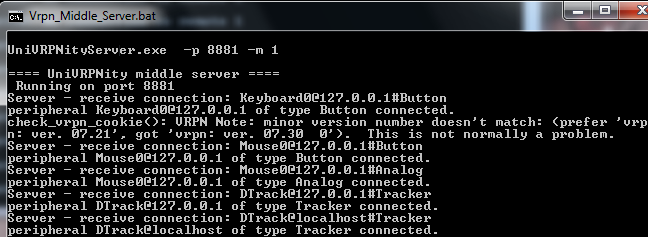
\includegraphics[scale=0.7]{UniVRPNityServer.png}
			\caption{UniVRPNity server at launch.}
		\end{center}
	\end{figure}


	\subsection{Communication}
	 Events are immediately binary serialize and transfer to client. However to avoid CPU eating, there is a sleep between 2 mainloop method call.

	\subsection{End}
	 It automatically close and kill a remote device when the associate socket is closed.
	
 	\subsection{Arguments of the server}
		\begin{itemize}
		      \item -h (--help) : Display help. Do not run the server
			\item -v (--verbose) : Display all peripheral event receive from VRPN server and send to the client
			\item -p (--port) : Specify the port number of the server. Default port is 8881
			\item -m (--millisleep) : Time between each internal mainloop in millisecond. Default time is 1ms
		\end{itemize}
		Example : UniVRPNityServer.exe -v -p 8881 -m 1

\section{UniVRPNity Client}

	\subsection{MonoBehaviour Scripts}
		These scripts are ready to use. You have to fill in network parameters and run Unity to recover peripheral data.
		\begin{itemize}
			\item Name : Device name which are specified in vrpn.cfg
			\item VRPN server IP : Host IP where are running a VRPN server
			\item UniVRPNity server IP : Host IP where are running a UniVRPNity server
			\item UniVRPNity server port : The port listened by UniVRPNity server
		\end{itemize}
				
		There are 3 specialized MonoBehaviour scripts :
		\begin{itemize}
			\item AnalogRemoteMB for analog device composed of channels
			\item ButtonRemoteMB for button device composed of states
			\item TrackerRemoteMB for tracker composed of position (Vector3) and orientation (Quaternion)
		\end{itemize}

		\subsubsection{AnalogRemoteMB example}
	
			\begin{figure}[H]
				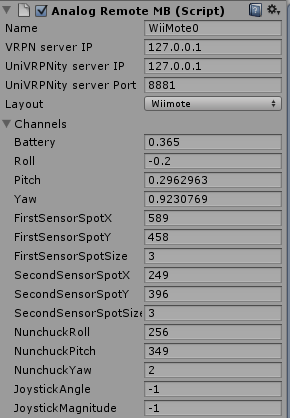
\includegraphics{AnalogWiimote.png}
				\caption{Monobehaviour remote of the Wiimote during execution.}
			\end{figure}

		\subsubsection{ButtonRemoteMB example}

			\begin{figure}[H]
				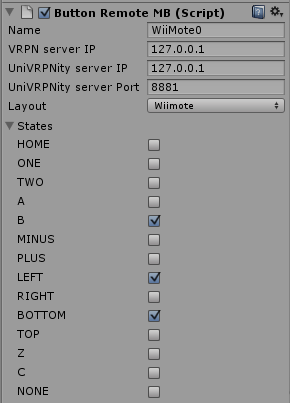
\includegraphics{ButtonWiimote.png}
				\caption{Monobehaviour remote of the Wiimote during execution.}
			\end{figure}


		\subsubsection{TrackerRemoteMB example}

			\begin{figure}[H]
				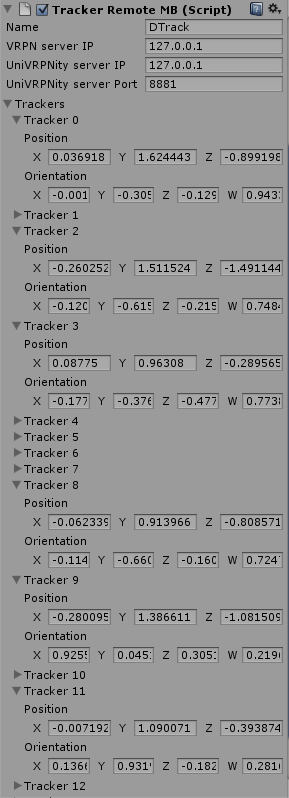
\includegraphics{TrackerDTrack.png}
				\caption{Monobehaviour remote of the DTrack during execution.}
			\end{figure}


\section{UniVRPNity Common}
	This library contains all server and client common elements : 
	\begin{itemize}
		\item Events which are sent over network
		\item Serializable Vector3 and Quaternion (conversion method are included)
		\item Some network default values
	\end{itemize}
	
\section{Known issues}

	\paragraph{Unity freezes at the beginning and throw lot of exceptions?} ~~\\
		Client have a long timeout for the server connection. It's happen when you forgot to run the UniVRPNity Server. If it's running, check address and port of the UniVRPNity server.
	
	\paragraph{Input values are not recovered?} ~~\\
		Check the VRPN server state. Is it running? Is the device enabled in VRPN configuration file. Use print device executable to test it. If it's correct, check the VRPN device name and it IP.
	
	\paragraph{Script stop recording information?} ~~\\
		If it happen, you can disable and enable the script to reconnect peripheral.

	
	\paragraph{UniVRPNity Server does not want to run} ~~\\
		Check if the used port is correct and available.

	
\section{Known bug}
	\begin{itemize}
		\item Date associate to event are wrong (wrong hour of the day). 
	\end{itemize}
	
\end{document}
